% Options for packages loaded elsewhere
\PassOptionsToPackage{unicode}{hyperref}
\PassOptionsToPackage{hyphens}{url}
\documentclass[
  ignorenonframetext,
]{beamer}
\newif\ifbibliography
\usepackage{pgfpages}
\setbeamertemplate{caption}[numbered]
\setbeamertemplate{caption label separator}{: }
\setbeamercolor{caption name}{fg=normal text.fg}
\beamertemplatenavigationsymbolsempty
% remove section numbering
\setbeamertemplate{part page}{
  \centering
  \begin{beamercolorbox}[sep=16pt,center]{part title}
    \usebeamerfont{part title}\insertpart\par
  \end{beamercolorbox}
}
\setbeamertemplate{section page}{
  \centering
  \begin{beamercolorbox}[sep=12pt,center]{section title}
    \usebeamerfont{section title}\insertsection\par
  \end{beamercolorbox}
}
\setbeamertemplate{subsection page}{
  \centering
  \begin{beamercolorbox}[sep=8pt,center]{subsection title}
    \usebeamerfont{subsection title}\insertsubsection\par
  \end{beamercolorbox}
}
% Prevent slide breaks in the middle of a paragraph
\widowpenalties 1 10000
\raggedbottom
\AtBeginPart{
  \frame{\partpage}
}
\AtBeginSection{
  \ifbibliography
  \else
    \frame{\sectionpage}
  \fi
}
\AtBeginSubsection{
  \frame{\subsectionpage}
}
\usepackage{iftex}
\ifPDFTeX
  \usepackage[T1]{fontenc}
  \usepackage[utf8]{inputenc}
  \usepackage{textcomp} % provide euro and other symbols
\else % if luatex or xetex
  \usepackage{unicode-math} % this also loads fontspec
  \defaultfontfeatures{Scale=MatchLowercase}
  \defaultfontfeatures[\rmfamily]{Ligatures=TeX,Scale=1}
\fi
\usepackage{lmodern}
\ifPDFTeX\else
  % xetex/luatex font selection
\fi
% Use upquote if available, for straight quotes in verbatim environments
\IfFileExists{upquote.sty}{\usepackage{upquote}}{}
\IfFileExists{microtype.sty}{% use microtype if available
  \usepackage[]{microtype}
  \UseMicrotypeSet[protrusion]{basicmath} % disable protrusion for tt fonts
}{}
\makeatletter
\@ifundefined{KOMAClassName}{% if non-KOMA class
  \IfFileExists{parskip.sty}{%
    \usepackage{parskip}
  }{% else
    \setlength{\parindent}{0pt}
    \setlength{\parskip}{6pt plus 2pt minus 1pt}}
}{% if KOMA class
  \KOMAoptions{parskip=half}}
\makeatother
\usepackage{longtable,booktabs,array}
\newcounter{none} % for unnumbered tables
\usepackage{calc} % for calculating minipage widths
\usepackage{caption}
% Make caption package work with longtable
\makeatletter
\def\fnum@table{\tablename~\thetable}
\makeatother
\usepackage{graphicx}
\makeatletter
\newsavebox\pandoc@box
\newcommand*\pandocbounded[1]{% scales image to fit in text height/width
  \sbox\pandoc@box{#1}%
  \Gscale@div\@tempa{\textheight}{\dimexpr\ht\pandoc@box+\dp\pandoc@box\relax}%
  \Gscale@div\@tempb{\linewidth}{\wd\pandoc@box}%
  \ifdim\@tempb\p@<\@tempa\p@\let\@tempa\@tempb\fi% select the smaller of both
  \ifdim\@tempa\p@<\p@\scalebox{\@tempa}{\usebox\pandoc@box}%
  \else\usebox{\pandoc@box}%
  \fi%
}
% Set default figure placement to htbp
\def\fps@figure{htbp}
\makeatother
\setlength{\emergencystretch}{3em} % prevent overfull lines
\providecommand{\tightlist}{%
  \setlength{\itemsep}{0pt}\setlength{\parskip}{0pt}}
% Slide layout defaults for warning-clean scientific decks.
\usepackage{etoolbox}
\IfFileExists{xurl.sty}{\usepackage{xurl}}{}
\IfFileExists{seqsplit.sty}{\usepackage{seqsplit}}{\newcommand{\seqsplit}[1]{#1}}
\protected\def\breakseq#1{\seqsplit{#1}}
\protected\def\breaktt#1{\begingroup\ttfamily\seqsplit{#1}\endgroup}
\setlength{\emergencystretch}{6em}
\tolerance=5000
\hbadness=10000
\hfuzz=1pt
\setlength{\tabcolsep}{2pt}
\AtBeginEnvironment{longtable}{\tiny\renewcommand{\arraystretch}{0.86}\setlength{\tabcolsep}{1pt}}
\AtBeginEnvironment{tabular}{\tiny\renewcommand{\arraystretch}{0.86}\setlength{\tabcolsep}{1pt}}

% Natbib and cross-reference fallbacks — slides don't load natbib
% or cleveref, but combined-PDF manuscript prose may emit these
% commands. The fallback renders citations as a bracketed key list
% and cross-references as detokenized labels so slides don't fail on
% undefined control sequences or raw underscores. \providecommand is
% a no-op if packages load later.
\providecommand{\citep}[1]{[#1]}
\providecommand{\citet}[1]{#1}
\providecommand{\citealp}[1]{#1}
\providecommand{\citeauthor}[1]{#1}
\providecommand{\citeyear}[1]{#1}
\providecommand{\cref}[1]{\texttt{\detokenize{#1}}}
\providecommand{\Cref}[1]{\texttt{\detokenize{#1}}}
\usepackage{bookmark}
\IfFileExists{xurl.sty}{\usepackage{xurl}}{} % add URL line breaks if available
\urlstyle{same}
% fallback for those not using the hyperref driver hyperxmp:
\makeatletter
\@ifundefined{xmpquote}{\newcommand{\xmpquote}[1]{#1}}{}
\makeatother
\hypersetup{
  hidelinks,
  pdfcreator={LaTeX via pandoc}}

\author{\texorpdfstring{}{}}
\date{}

\begin{document}

\begin{frame}[fragile,allowframebreaks]{Results}
\protect\phantomsection\label{results}
\begin{block}{Grammar product space}
\protect\phantomsection\label{grammar-product-space}
{\def\LTcaptype{none} % do not increment counter
\begin{longtable}[]{@{}
  >{\raggedright\arraybackslash}p{(\linewidth - 4\tabcolsep) * \real{0.3333}}
  >{\raggedright\arraybackslash}p{(\linewidth - 4\tabcolsep) * \real{0.3333}}
  >{\raggedright\arraybackslash}p{(\linewidth - 4\tabcolsep) * \real{0.3333}}@{}}
\toprule\noalign{}
\begin{minipage}[b]{\linewidth}\raggedright
Slot
\end{minipage} & \begin{minipage}[b]{\linewidth}\raggedright
Options
\end{minipage} & \begin{minipage}[b]{\linewidth}\raggedright
Values
\end{minipage} \\
\midrule\noalign{}
\endhead
primitive\_domain & 5 & optimization, dynamics, statistics, signal,
graph \\
track & 3 & analytical, empirical, hybrid \\
section\_set & 3 & minimal, standard, extended \\
figure\_profile & 2 & minimal, full \\
qr\_profile & 2 & off, on \\
integrity\_profile & 2 & sha256, merkle \\
\bottomrule\noalign{}
\end{longtable}
}

\begin{figure}
\centering
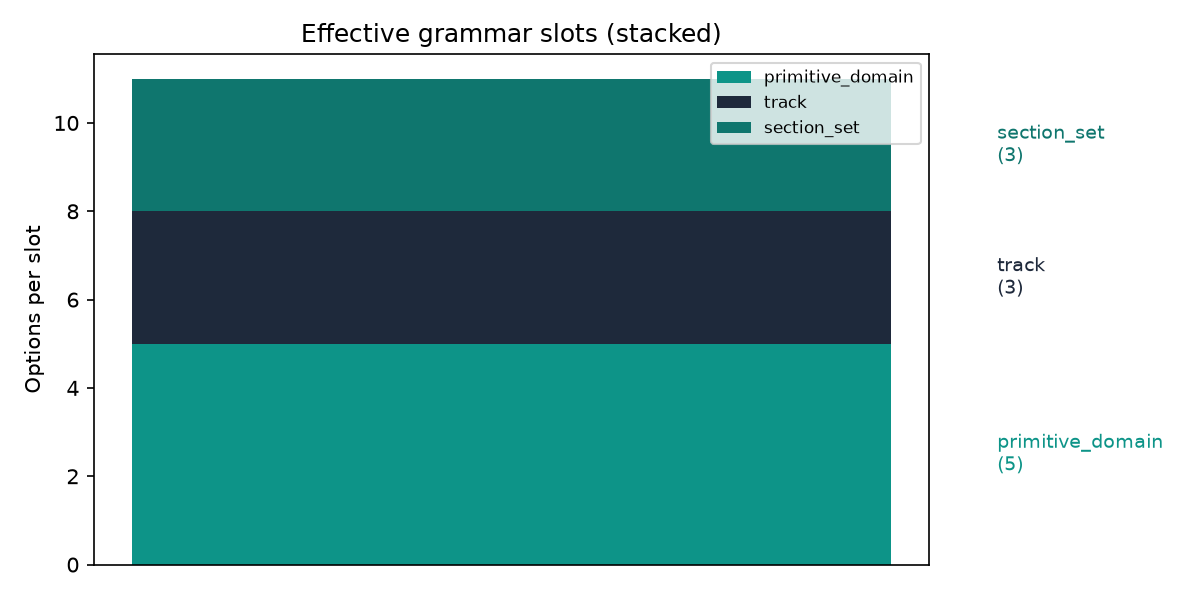
\includegraphics[width=0.85\linewidth,height=0.46\textheight,keepaspectratio,alt={Options per grammar slot, stacked. Each band is one slot's contribution to the total product size; three bands are reserved (presentational/sealing) and are excluded from the effective product space discussed below.}]{../figures/fig_stacked_product.png}
\caption{Options per grammar slot, stacked. Each band is one slot's
contribution to the total product size; three bands are reserved
(presentational/sealing) and are excluded from the effective product
space discussed below.}\label{fig:stacked_product}
\end{figure}

\begin{itemize}
\tightlist
\item
  \textbf{Total product size}: 360 cells
\item
  \textbf{Effective product size} (reserved slots excluded): 45 cells
\item
  \textbf{Reserved slots} (3):
  \breaktt{figure\_profile,\ qr\_profile,\ integrity\_profile}
\end{itemize}

\begin{figure}
\centering
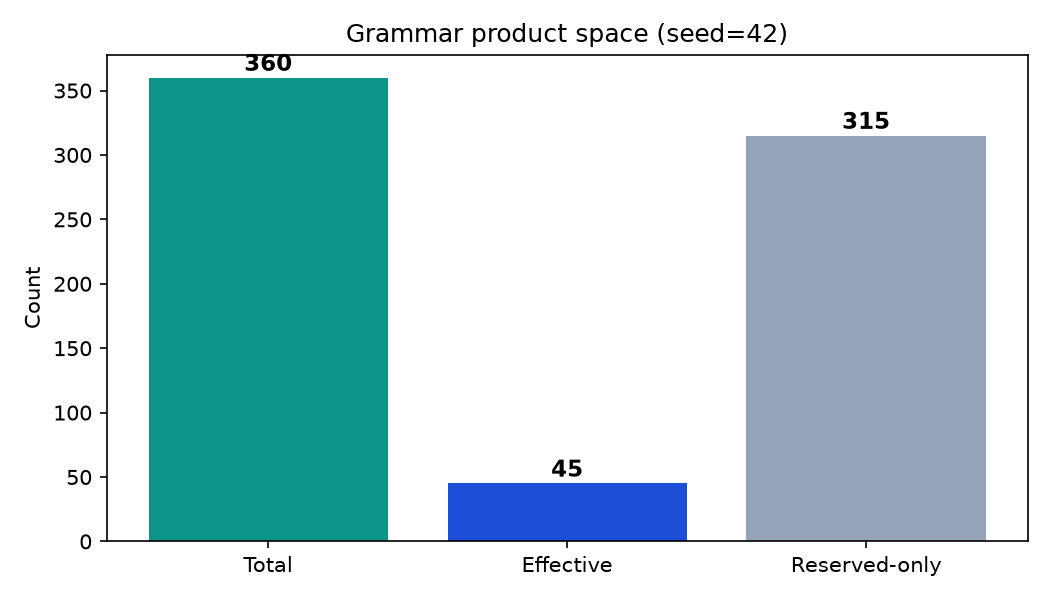
\includegraphics[width=0.8\linewidth,height=0.46\textheight,keepaspectratio,alt={Total, effective, and reserved-only product size for the grammar at seed=42, generated by fig\_product\_space\_annotation (src/manuscript\_figures.py) directly from Grammar.product\_size / Grammar.effective\_product\_size --- not hand-typed.}]{../figures/fig_product_space.png}
\caption{Total, effective, and reserved-only product size for the
grammar at seed=42, generated by
\protect\breaktt{fig\_product\_space\_annotation}
(\protect\breaktt{src/manuscript\_figures.py}) directly from
\protect\breaktt{Grammar.product\_size} /
\protect\breaktt{Grammar.effective\_product\_size} --- not
hand-typed.}\label{fig:product_space}
\end{figure}

Every row in the table above is a \texttt{GrammarSlot} parsed from
\breaktt{manuscript/config.yaml} by \texttt{parse\_grammar()}
(\texttt{src/grammar.py}). Each slot contributes a multiplicative factor
to \breaktt{Grammar.product\_size}, which is the raw cross-product of all
option counts --- not an estimate, but the literal
\breaktt{n\ *=\ len(s.options)} accumulation over every slot. The
\breaktt{Grammar.grammar\_hash} property serialises the seed, every slot
name, and every option list into a canonical JSON string
(\texttt{canonical()}) and takes the first sixteen hex characters of its
SHA-256 digest --- \breaktt{f84a8f9dbcb18e37} for the grammar as
currently checked into this project. Any edit to a slot's option list,
the addition or removal of a slot, or a change to the seed changes this
hash deterministically; it is not a version string maintained by hand.

The six slots split into two categories. Three are
\emph{content-determining}: \breaktt{primitive\_domain} selects which of
the five kernel modules described below is copied into the child
project, \texttt{track} selects the manuscript's analytical posture
(\texttt{analytical}, \texttt{empirical}, or \texttt{hybrid}), and
\texttt{section\_set} selects which subset of manuscript sections is
rendered (\texttt{minimal}, \texttt{standard}, or \texttt{extended}).
The remaining three --- \texttt{figure\_profile}, \texttt{qr\_profile},
and \breaktt{integrity\_profile} --- are declared in
\texttt{RESERVED\_SLOTS} (\texttt{src/grammar.py}) and govern only
\emph{presentational and sealing} behaviour: how many figures are
generated, whether the sealed payload is rendered as a QR PNG, and
whether the provenance hash is a flat SHA-256 or a Merkle root over
per-file hashes (\breaktt{src/integrity.py::merkle\_root}). None of the
three reserved slots changes which primitive kernel runs or what its
output is, which is exactly why
\breaktt{Grammar.effective\_product\_size} --- the number that matters
when asking ``how many \emph{scientifically distinct} children can this
grammar produce'' --- divides the reserved slots back out. The ratio
between the total and effective product sizes above is, by construction,
the product of the three reserved slots' own option counts; no other
slot is capable of changing that ratio.
\end{block}

\begin{block}{Effective slot breakdown}
\protect\phantomsection\label{effective-slot-breakdown}
{\def\LTcaptype{none} % do not increment counter
\begin{longtable}[]{@{}
  >{\raggedright\arraybackslash}p{(\linewidth - 4\tabcolsep) * \real{0.3333}}
  >{\raggedright\arraybackslash}p{(\linewidth - 4\tabcolsep) * \real{0.3333}}
  >{\raggedright\arraybackslash}p{(\linewidth - 4\tabcolsep) * \real{0.3333}}@{}}
\toprule\noalign{}
\begin{minipage}[b]{\linewidth}\raggedright
Slot
\end{minipage} & \begin{minipage}[b]{\linewidth}\raggedright
Options
\end{minipage} & \begin{minipage}[b]{\linewidth}\raggedright
Values
\end{minipage} \\
\midrule\noalign{}
\endhead
primitive\_domain & 5 & optimization, dynamics, statistics, signal,
graph \\
track & 3 & analytical, empirical, hybrid \\
section\_set & 3 & minimal, standard, extended \\
\bottomrule\noalign{}
\end{longtable}
}

\breaktt{grammar.effective\_slots} (\texttt{src/grammar.py}) is exactly
\texttt{grammar.slots} filtered against \texttt{RESERVED\_SLOTS} --- the
same list rendered in the previous section, minus the three
sealing/presentation dimensions. This is the space a reviewer should
reason about when asking whether the grammar is a meaningful generator
rather than a combinatorial trick that multiplies unrelated toggles: 5
primitive domains times three narrative tracks times three section-set
sizes is the actual space of scientifically distinguishable children
this template can emit.
\end{block}

\begin{block}{The five primitive domains}
\protect\phantomsection\label{the-five-primitive-domains}
\begin{figure}
\centering
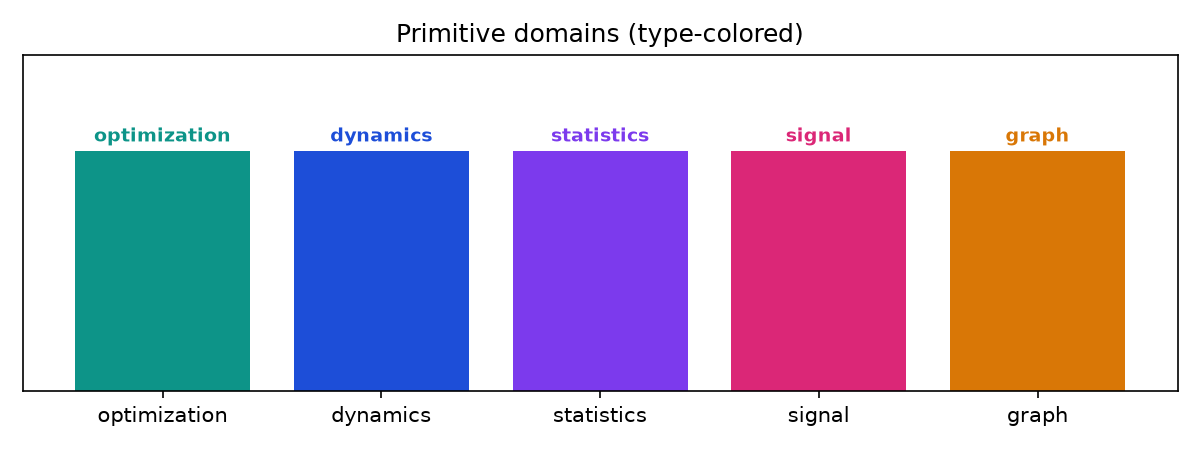
\includegraphics[width=0.85\linewidth,height=0.46\textheight,keepaspectratio,alt={The five primitive domains, type-colored: optimization, dynamics, statistics, signal, graph.}]{../figures/fig_domain_coverage.png}
\caption{The five primitive domains, type-colored:
\protect\texttt{optimization}, \protect\texttt{dynamics},
\protect\texttt{statistics}, \protect\texttt{signal},
\protect\texttt{graph}.}\label{fig:domain_coverage}
\end{figure}

Each domain in
\breaktt{-\ optimization\ -\ dynamics\ -\ statistics\ -\ signal\ -\ graph}
is a Python module under \texttt{src/primitives/} exporting a
\texttt{PRIMITIVES:\ tuple{[}PrimitiveSpec,\ ...{]}} collected by
\breaktt{collect\_primitives()}
(\breaktt{src/primitives/\_\_init\_\_.py}). A \texttt{PrimitiveSpec}
(\breaktt{src/primitives/base.py}) bundles a callable kernel, an example
input, an expected output (or \texttt{None} when the check is structural
rather than a fixed value), a numerical tolerance, and --- for five of
the eight kernels --- a \breaktt{negative\_control} callable whose entire
purpose is to fail the primary kernel's own success criterion.
\breaktt{collect\_primitives()} returns exactly the five domains named
above (\breaktt{test\_collect\_primitives\_expected\_modules}) and a
total of eight primitive kernels across them
(\breaktt{test\_total\_primitive\_count}): two in \texttt{optimization},
one in \texttt{dynamics}, one in \texttt{statistics}, two in
\texttt{signal}, and two in \texttt{graph}.

\textbf{Optimization.} \breaktt{gradient\_descent}
(\breaktt{src/primitives/optimization.py}) runs explicit gradient descent
on the convex quadratic \texttt{f(x)\ =\ 0.5\ (x-c)\^{}T\ A\ (x-c)},
whose gradient is \texttt{A(x-c)}. Because the problem is convex
quadratic, its analytic minimiser is known in closed form ---
\texttt{x*\ =\ c}, computed independently by the sibling kernel
\breaktt{analytic\_minimizer} --- so the iterative and closed-form
solutions can be cross-checked against each other rather than against a
single hardcoded expectation. On the example input (a diagonal
\texttt{A}, \texttt{c\ =\ (1,\ -1)}, 200 steps at learning rate 0.1) the
two agree to within \texttt{1e-4}. The domain's negative control,
\breaktt{\_negative\_control\_wrong\_sign}, is the same loop with the
gradient step's sign flipped (\breaktt{x\ =\ x\ +\ lr\ *\ grad} instead
of \breaktt{x\ =\ x\ -\ lr\ *\ grad}); this turns descent into ascent and
diverges away from \texttt{c} instead of converging to it, giving the
mutation gate (see Honesty Contract) something to detect if the sign
were ever silently restored to ``wrong.''

\textbf{Dynamics.} \breaktt{damped\_oscillator}
(\breaktt{src/primitives/dynamics.py}) integrates the damped harmonic
oscillator ODE
\texttt{x\textquotesingle{}\textquotesingle{}\ +\ 2*zeta*omega*x\textquotesingle{}\ +\ omega\^{}2*x\ =\ 0}
with explicit Euler stepping, and separately computes the closed-form
under-damped envelope \breaktt{x0\ *\ exp(-zeta*omega*t)}. The test suite
does not merely check that the two arrays are close; it checks four
independent structural properties of the same trajectory: the numerical
amplitude stays inside the analytical envelope plus a 5\% Euler-error
tolerance
(\breaktt{test\_damped\_oscillator\_amplitude\_bounded\_by\_envelope}),
the envelope itself is monotonically non-increasing
(\breaktt{test\_damped\_oscillator\_envelope\_monotone\_decreasing}),
heavy damping drives the trajectory near zero by the end of the run
(\breaktt{test\_damped\_oscillator\_decays\_to\_near\_zero}), and the
initial condition is reproduced exactly. The negative control,
\breaktt{\_zero\_damping\_control}, re-runs the same integrator with
\texttt{zeta} forced to zero; its envelope is flat at \texttt{x0} rather
than decaying, and \breaktt{test\_zero\_damping\_envelope\_flat} checks
that flatness directly --- so a broken damping term that decayed
regardless of the damping value would be caught, not just a broken
damping term that fails to decay at all.

\textbf{Statistics.} \texttt{ols\_fit}
(\breaktt{src/primitives/statistics.py}) solves ordinary least squares
via the normal equations,
\texttt{beta\_hat\ =\ (X\^{}T\ X)\^{}\{-1\}\ X\^{}T\ y}, solved with
\breaktt{numpy.linalg.solve} rather than an explicit matrix inverse. The
example input is synthetic, not observational: fifty rows with an
intercept column and one Gaussian covariate
(\breaktt{rng\ =\ np.random.default\_rng(42)}), a fixed true coefficient
vector \breaktt{beta\ =\ (2.0,\ -3.0)}, and additive noise scaled to
\texttt{0.1} standard deviations. Because the data-generating
coefficients are known by construction, recovery is checked directly ---
\breaktt{test\_ols\_fit\_recovers\_beta} requires the estimated and true
beta to agree within Euclidean distance \texttt{0.1} --- alongside an R²
floor of \texttt{0.95} and a near-zero mean residual. The negative
control, \breaktt{\_shuffled\_control}, permutes the \texttt{y} labels
with an independently seeded generator
(\breaktt{rng\ =\ np.random.default\_rng(0)}) before fitting; breaking
the true \texttt{X}-\texttt{y} correspondence this way is asserted to
drop R² below \texttt{0.5}
(\breaktt{test\_shuffled\_control\_poor\_r\_squared}), giving a concrete,
falsifiable bound on how badly a shuffled fit \emph{should} perform.

\textbf{Signal.} This domain carries two kernels validated by structural
properties rather than fixed target arrays, since \texttt{expected=None}
for both. \texttt{dft} computes the Discrete Fourier Transform directly
as a matrix-vector product against the exponential basis matrix
\breaktt{exp(-2j*pi*k*n/N)} --- an explicit \texttt{O(N\^{}2)}
construction, not a call into \texttt{numpy.fft}. Its correctness is
checked by Parseval's theorem
(\texttt{sum(\textbar{}X{[}k{]}\textbar{}\^{}2)\ ==\ N\ *\ sum(\textbar{}x{[}n{]}\textbar{}\^{}2)}
to within a relative tolerance of \texttt{1e-6}) and by recovering the
correct dominant frequency bin (index 5, positive or negative) from a
pure 5 Hz sinusoid sampled at 64 points. \texttt{convolve\_known} wraps
\texttt{numpy.convolve} with a fixed three-tap smoothing kernel,
\texttt{{[}0.25,\ 0.5,\ 0.25{]}}; its own test suite checks that
smoothing cannot increase variance
(\breaktt{test\_convolve\_known\_smoothing\_reduces\_variance}). Its
negative control, \breaktt{\_identity\_kernel\_convolve}, substitutes the
identity kernel \texttt{{[}1.0{]}} under \texttt{mode="same"}, which by
the definition of convolution must reproduce the input signal exactly
(\texttt{atol=1e-12}) --- a stronger, algebraically-derived check than
an arbitrary ``looks different'' comparison.

\textbf{Graph.} \texttt{bfs\_distances}
(\breaktt{src/primitives/graph.py}) computes shortest-path distances on a
fixed five-node undirected graph (\texttt{A}--\texttt{E}, encoded as an
adjacency dict) via a plain breadth-first queue. Because the graph is
fixed and small, the expected distances from source \texttt{A} are
enumerable by hand and are asserted exactly:
\texttt{\{A:\ 0,\ B:\ 1,\ C:\ 1,\ D:\ 2,\ E:\ 3\}}, with tolerance
\texttt{0.0}. Its negative control, \breaktt{\_disconnected\_control},
replaces the adjacency of the source node with an empty list, collapsing
the reachable set to the source alone --- a graph-structural way of
breaking the primitive rather than perturbing a numeric input.
\texttt{pagerank} runs the standard power-iteration update with damping
\texttt{0.85} over 50 iterations, redistributing dangling nodes' rank
mass evenly rather than dropping it. It has no single fixed expected
output --- rank values depend on iteration count and are not
hand-derivable --- so it is instead validated by three invariants any
correct PageRank computation must satisfy regardless of the specific
graph: ranks sum to \texttt{1.0} within \texttt{1e-6}, every node in the
graph receives a rank entry, and every rank is strictly positive
(ensured by the \texttt{(1-damping)/n} teleportation floor added at
every iteration).

Across the five domains, five of the eight primitives carry an explicit
negative control; the remaining three (\breaktt{analytic\_minimizer},
\texttt{dft}, and \texttt{pagerank}) are validated purely through
cross-checks against an independent computation or through algebraic
invariants (Parseval's theorem, PageRank's stochastic-normalization
property) that a broken implementation would be unlikely to satisfy by
accident. This mirrors the property-based testing tradition
\breakseq{[@claessen2000quickcheck; @maciver2019hypothesis]}: rather than
asserting a single hand-picked input/output pair, the suite asserts
properties that must hold across a class of inputs --- the same style
used at the grammar level in
\breaktt{tests/test\_property\_invariants.py}, where
\texttt{hypothesis}-generated seeds are used to check, for every seed
drawn, that \texttt{product\_size} really is the product of option
counts and that \breaktt{effective\_product\_size} does not exceed it.
\end{block}

\begin{block}{Exemplar generation}
\protect\phantomsection\label{exemplar-generation}
Running
\breaktt{uv\ run\ python\ scripts/autopoiesis.py\ expand\ -\/-seed\ 42}
produces a spec with \breaktt{primitive\_domain} deterministically
selected from the grammar.

All 5 domains successfully materialize runnable child projects. Each
child project:

\begin{enumerate}
\tightlist
\item
  Contains a \texttt{primitives/} package with the selected kernel.
\item
  Runs \texttt{analysis.py} without error.
\item
  Has a \texttt{provenance.json} that passes \texttt{verify\_child}.
\item
  Passes all child-level smoke tests.
\end{enumerate}
\end{block}

\begin{block}{Test results}
\protect\phantomsection\label{test-results}
\begin{itemize}
\tightlist
\item
  \textbf{Test count}: 493
\item
  \textbf{Coverage}: 96.28\%
\item
  \textbf{Grammar hash}: \breaktt{f84a8f9dbcb18e37}
\end{itemize}

Both the test count and coverage percentage above are produced by
\breaktt{measure\_test\_summary()}
(\breaktt{src/manuscript\_variables.py}), which shells out to this
project's own \texttt{pytest} + \texttt{coverage} run
(\texttt{-\/-cov-branch}, matching the repository-root branch-coverage
methodology) against \texttt{tests/} and \texttt{src/} and parses the
real \texttt{passed} count and \texttt{coverage.json} totals from that
subprocess. There is no fallback literal: if the subprocess fails, times
out, or its output fails to parse, both fields resolve to the string
\texttt{"pending"} rather than a plausible-looking number --- the same
discipline that governs every other numeric token in this manuscript.

\begin{figure}
\centering
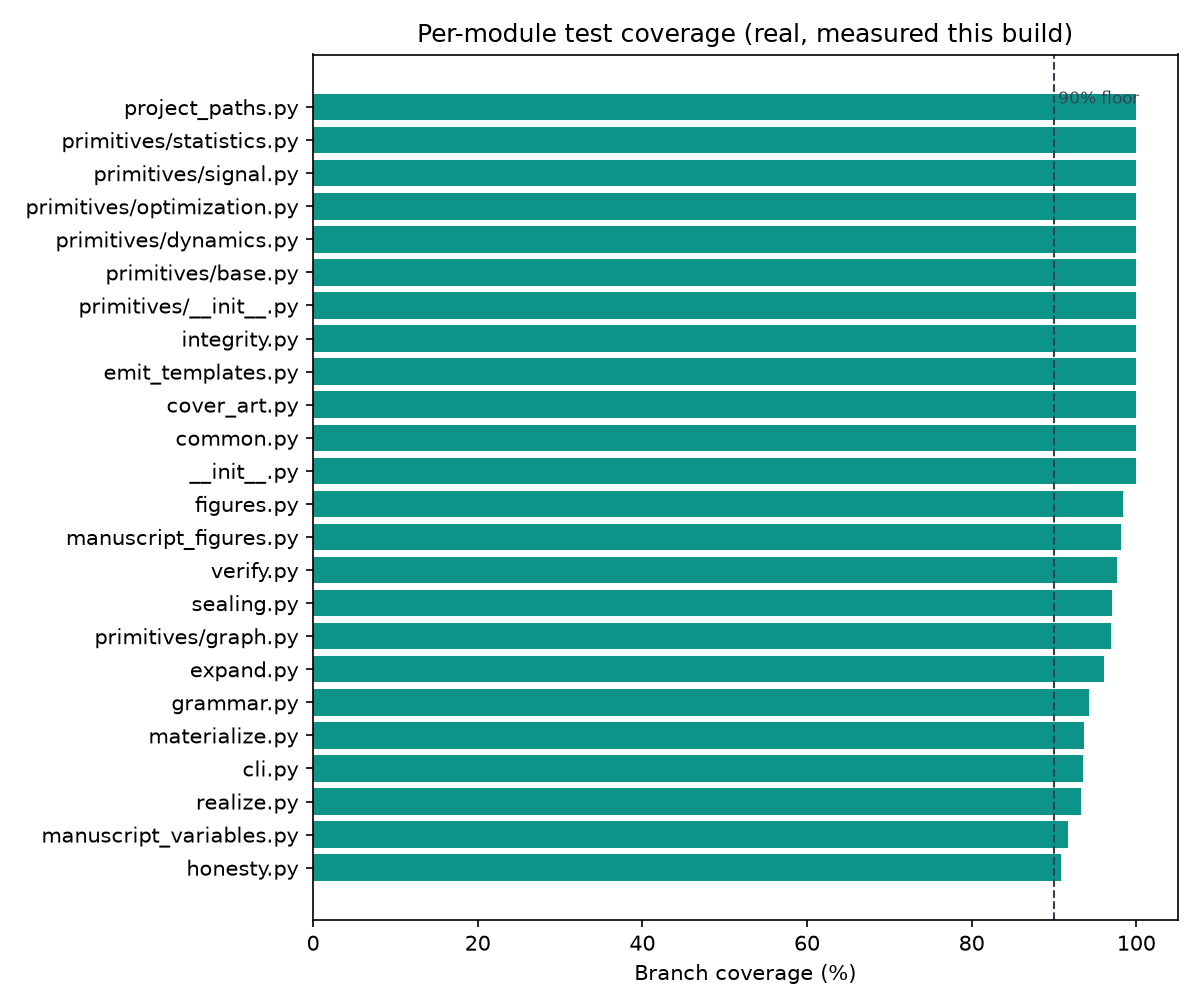
\includegraphics[width=0.9\linewidth,height=0.46\textheight,keepaspectratio,alt={Real, per-module branch coverage from the same measurement run that produces 493/96.28 above --- not an aggregate alone. Any module below the repository's 90\% floor would be drawn in red rather than smoothed into the headline percentage; none is, in this measurement.}]{../figures/fig_coverage_by_module.png}
\caption{Real, per-module branch coverage from the same measurement run
that produces 493/96.28 above --- not an aggregate alone. Any module
below the repository's 90\% floor would be drawn in red rather than
smoothed into the headline percentage; none is, in this
measurement.}\label{fig:coverage_by_module}
\end{figure}

The aggregate 96.28\% is a mean weighted by statement and branch count,
not a uniform floor --- \breakseq{[@fig:coverage\_by\_module]} shows the real
spread. As of this measurement every module clears the 90\% line;
\texttt{common.py} and \texttt{cover\_art.py} sit at 100\% and
\texttt{figures.py} at 98.41\% after closing what were, in an earlier
draft of this manuscript, the three lowest-coverage modules (see
\texttt{CHANGELOG.md}'s Wave 10 entry for the specific branches that
were untested and the tests added to close them); every module under
\texttt{src/primitives/} and the honesty/integrity core sit at or near
100\%. Both the aggregate number and this per-module breakdown are read
from the same persisted \breaktt{output/data/coverage\_full.json} --- a
single generator run, not two separately-computed views that could
silently drift apart. This is a snapshot, not a permanent state:
coverage moves as tests are added or code changes, and
\breakseq{[@fig:coverage\_by\_module]} should be regenerated
(\breaktt{stage\_02\_analysis.py}) rather than trusted from a prior
render whenever that question matters.
\end{block}
\end{frame}

\end{document}
